\documentclass[aspectratio=169,11pt]{beamer}

% ============================================================
% PACKAGES
% ============================================================
\usepackage{graphicx}
\usepackage{tikz}
\usetikzlibrary{positioning,arrows.meta}
\usepackage{xcolor}
\usepackage{booktabs}
\usepackage{tabularx}
\usepackage{array}
\usepackage{ragged2e}
\usepackage{hyperref}

% ============================================================
% COLORS - SAME AS PHASE-I
% ============================================================
\definecolor{GEUBlue}{RGB}{20,55,105}
\definecolor{GEULightBlue}{RGB}{238,244,251}
\definecolor{GEUGrey}{RGB}{90,90,90}
\definecolor{GEULightGrey}{RGB}{245,246,248}

% ============================================================
% BEAMER SETTINGS
% ============================================================
\usetheme{default}
\setbeamertemplate{navigation symbols}{}
\setbeamertemplate{blocks}[rounded][shadow=false]

\setbeamercolor{normal text}{fg=black,bg=white}
\setbeamercolor{frametitle}{fg=GEUBlue}
\setbeamercolor{structure}{fg=GEUBlue}
\setbeamercolor{block title}{fg=GEUBlue,bg=GEULightBlue}
\setbeamercolor{block body}{fg=black,bg=GEULightBlue}

\setbeamerfont{frametitle}{size=\Large,series=\bfseries}

% ============================================================
% LOGO
% ============================================================
% Upload the Graphic Era logo with this filename to Overleaf.
\newcommand{\GEULogo}{graphicera_logo.png}

% ============================================================
% HEADER
% ============================================================
\setbeamertemplate{headline}{%
  \begin{tikzpicture}[remember picture,overlay]
    \node[
        anchor=north east,
        xshift=-0.30cm,
        yshift=-0.12cm
    ] at (current page.north east)
    {\includegraphics[height=0.62cm]{\GEULogo}};
  \end{tikzpicture}
  \vspace{0.72cm}
}

% ============================================================
% FRAME TITLE
% ============================================================
\setbeamertemplate{frametitle}{%
  \vspace{0.03cm}
  \insertframetitle\par
  \vspace{0.04cm}
  \textcolor{GEUBlue}{\rule{\textwidth}{0.9pt}}
  \vspace{0.03cm}
}

% ============================================================
% FOOTER
% ============================================================
\setbeamertemplate{footline}{%
  \leavevmode
  \hbox{%
  \begin{beamercolorbox}[
      wd=.82\paperwidth,
      ht=0.32cm,
      dp=0.10cm,
      leftskip=.3cm
  ]{author in head/foot}
    \tiny Department of Computer Science \& Engineering |
    Graphic Era (Deemed to be University)
  \end{beamercolorbox}%
  \begin{beamercolorbox}[
      wd=.18\paperwidth,
      ht=0.32cm,
      dp=0.10cm,
      rightskip=.3cm
  ]{date in head/foot}
    \hfill\tiny\insertframenumber/\inserttotalframenumber
  \end{beamercolorbox}}
}

% ============================================================
% CUSTOM COMMANDS
% ============================================================
\newcommand{\smallnote}[1]{%
\vspace{0.08cm}
{\scriptsize\color{GEUGrey}#1}
}

\newcommand{\placeholder}[1]{%
\textit{\color{GEUGrey}#1}
}

% ============================================================
% DOCUMENT INFORMATION
% ============================================================
\title{\textbf{Project-Based Learning}\\[2mm]\large Phase-II Evaluation}
\author{\textbf{Project Title}\\Team ID: XXXX}

\institute{
Department of Computer Science \& Engineering\\
Graphic Era (Deemed to be University), Dehradun
}

\date{Academic Session 2026--27}

% ============================================================
% DOCUMENT
% ============================================================
\begin{document}

% ============================================================
% SLIDE 1
% ============================================================
\begin{frame}[plain]

\begin{tikzpicture}[remember picture,overlay]

\draw[GEUBlue,line width=3pt]
(current page.north west) -- (current page.north east);

\node[
    anchor=north east,
    xshift=-0.45cm,
    yshift=-0.35cm
] at (current page.north east)
{\includegraphics[height=1.0cm]{\GEULogo}};

\node[
    align=center,
    text width=.84\paperwidth
] at ([yshift=.25cm]current page.center)
{
{\color{GEUBlue}
\fontsize{26}{30}\selectfont
\bfseries PROJECT-BASED LEARNING}
\\[3mm]

{\fontsize{18}{22}\selectfont
PHASE-II EVALUATION}
\\[7mm]

{\color{GEUGrey}
\Large\bfseries
\placeholder{Project Title}}
\\[3mm]

{\color{GEUBlue}
\normalsize Team ID: XXXX}
};

\node[
    align=center,
    anchor=south,
    yshift=.42cm
] at (current page.south)
{
\bfseries
Department of Computer Science \& Engineering\\
Graphic Era (Deemed to be University), Dehradun\\[-1mm]
\scriptsize Academic Session 2026--27
};

\end{tikzpicture}

\end{frame}

% ============================================================
% SLIDE 2
% ============================================================
\begin{frame}{Team \& Mentor Details}

\begin{columns}[T,totalwidth=\textwidth]

\column{.48\textwidth}

\begin{block}{Team Information}
\begin{tabular}{@{}ll@{}}
\textbf{Team ID:} & XXXX\\
\textbf{Semester:} & 3rd / 5th\\
\textbf{Section:} & XX\\
\textbf{Domain:} & \placeholder{XXXX}
\end{tabular}
\end{block}

\column{.48\textwidth}

\begin{block}{Team Members}
1.\quad \placeholder{Student Name -- ID}\\
2.\quad \placeholder{Student Name -- ID}\\
3.\quad \placeholder{Student Name -- ID}\\
4.\quad \placeholder{Student Name -- ID}
\end{block}

\end{columns}

\vspace{2mm}

\begin{block}{Mentor}
\placeholder{Dr. / Mr. / Ms. Mentor Name}
\hfill
\textbf{Interactions completed:}
\underline{\hspace{12mm}}
\end{block}

\vfill

\smallnote{
Brief Discussion: Introduce the team, project domain, mentor,
and responsibilities of the team members.
}

\end{frame}

% ============================================================
% SLIDE 3
% ============================================================
\begin{frame}{Phase-I Recap \& Feedback Incorporated}

\begin{block}{Phase-I Status}
\placeholder{
Briefly summarize what was proposed and achieved during Phase-I.
}
\end{block}

\vspace{2mm}

\begin{columns}[T,totalwidth=\textwidth]

\column{.48\textwidth}

\textbf{\color{GEUBlue}Feedback Received}

\begin{itemize}\itemsep2pt
\item \placeholder{Suggestion / Feedback 1}
\item \placeholder{Suggestion / Feedback 2}
\item \placeholder{Suggestion / Feedback 3}
\end{itemize}

\column{.48\textwidth}

\textbf{\color{GEUBlue}Changes Incorporated}

\begin{itemize}\itemsep2pt
\item \placeholder{Modification 1}
\item \placeholder{Modification 2}
\item \placeholder{Modification 3}
\end{itemize}

\end{columns}

\vfill

\smallnote{
Brief Discussion: Explain the major feedback received during Phase-I
and clearly demonstrate how it has been incorporated.
}

\end{frame}

% ============================================================
% SLIDE 4
% ============================================================
\begin{frame}{Problem Statement \& Finalized Objectives}

\begin{block}{Problem Statement}
\placeholder{
State the finalized problem being addressed after incorporating
Phase-I feedback.
}
\end{block}

\vspace{2mm}

\textbf{\color{GEUBlue}Finalized Objectives}

\begin{enumerate}\itemsep3pt
\item \placeholder{Objective 1}
\item \placeholder{Objective 2}
\item \placeholder{Objective 3}
\item \placeholder{Objective 4}
\end{enumerate}

\vfill

\smallnote{
Brief Discussion: Avoid repeating the complete Phase-I presentation.
Focus on the finalized problem, scope and measurable objectives.
}

\end{frame}

% ============================================================
% SLIDE 5
% ============================================================
\begin{frame}{Updated System Architecture / Workflow}

\begin{center}

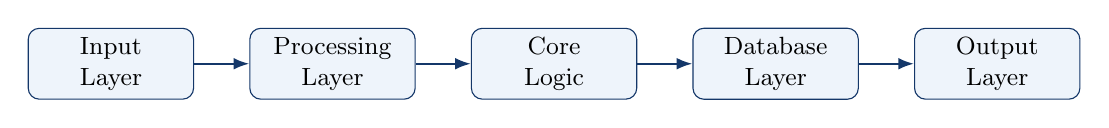
\begin{tikzpicture}[
node distance=7mm,
box/.style={
rectangle,
rounded corners,
draw=GEUBlue,
fill=GEULightBlue,
minimum width=2.10cm,
minimum height=9mm,
align=center,
font=\small
},
arrow/.style={
-{Latex[length=2mm]},
thick,
draw=GEUBlue
}
]

\node[box] (a) {Input\\Layer};
\node[box,right=of a] (b) {Processing\\Layer};
\node[box,right=of b] (c) {Core\\Logic};
\node[box,right=of c] (d) {Database\\Layer};
\node[box,right=of d] (e) {Output\\Layer};

\draw[arrow] (a)--(b);
\draw[arrow] (b)--(c);
\draw[arrow] (c)--(d);
\draw[arrow] (d)--(e);

\end{tikzpicture}

\end{center}

\vspace{4mm}

\begin{columns}[T,totalwidth=\textwidth]

\column{.48\textwidth}

\textbf{\color{GEUBlue}Major Components}

\begin{itemize}\itemsep2pt
\item \placeholder{Component 1}
\item \placeholder{Component 2}
\item \placeholder{Component 3}
\end{itemize}

\column{.48\textwidth}

\textbf{\color{GEUBlue}Changes Since Phase-I}

\begin{itemize}\itemsep2pt
\item \placeholder{Architecture change}
\item \placeholder{New component}
\item \placeholder{Improved workflow}
\end{itemize}

\end{columns}

\vfill

\smallnote{
Brief Discussion: Present the updated architecture and explain
how individual modules communicate with each other.
}

\end{frame}

% ============================================================
% SLIDE 6
% ============================================================
\begin{frame}{Module Design \& Functional Requirements}

\begin{columns}[T,totalwidth=\textwidth]

\column{.48\textwidth}

\textbf{\color{GEUBlue}Major Modules}

\begin{enumerate}\itemsep3pt
\item \placeholder{Module 1}
\item \placeholder{Module 2}
\item \placeholder{Module 3}
\item \placeholder{Module 4}
\end{enumerate}

\column{.48\textwidth}

\textbf{\color{GEUBlue}Functional Requirements}

\begin{itemize}\itemsep3pt
\item \placeholder{Functional Requirement 1}
\item \placeholder{Functional Requirement 2}
\item \placeholder{Functional Requirement 3}
\item \placeholder{Functional Requirement 4}
\end{itemize}

\end{columns}

\vfill

\begin{block}{Module Dependency}
\placeholder{
Briefly describe dependencies and interactions between major modules.
}
\end{block}

\smallnote{
Brief Discussion: Explain what each module does and how it contributes
to the complete system.
}

\end{frame}

% ============================================================
% SLIDE 7
% ============================================================
\begin{frame}{Technology Stack \& Development Methodology}

\begin{columns}[T,totalwidth=\textwidth]

\column{.48\textwidth}

\begin{block}{Technology Stack}

\begin{itemize}\itemsep2pt
\item Programming: \placeholder{C / C++ / Other}
\item Database: \placeholder{MySQL / PostgreSQL}
\item Framework: \placeholder{XXXX}
\item Development Tool: \placeholder{XXXX}
\item Version Control: \placeholder{Git / GitHub}
\end{itemize}

\end{block}

\column{.48\textwidth}

\begin{block}{Development Methodology}

\begin{enumerate}\itemsep2pt
\item Requirement Analysis
\item System Design
\item Module Development
\item Integration
\item Testing \& Validation
\end{enumerate}

\end{block}

\end{columns}

\vfill

\smallnote{
Brief Discussion: Explain why the selected technologies are appropriate
and how the team is following the development methodology.
}

\end{frame}

% ============================================================
% SLIDE 8
% ============================================================
\begin{frame}{Implementation of PBL Course Concepts}

\scriptsize

\begin{center}

\renewcommand{\arraystretch}{1.25}

\begin{tabularx}{.96\textwidth}
{@{}>{\bfseries}p{3.0cm}X p{2.5cm}@{}}

\toprule
Course & Concepts Actually Implemented & Project Module\\
\midrule

Data Structures in C &
\placeholder{Arrays, Linked Lists, Trees, Graphs, Hashing, etc.} &
\placeholder{Module X}\\

OOPs with C++ &
\placeholder{Classes, Inheritance, Polymorphism, STL, etc.} &
\placeholder{Module Y}\\

\midrule

Operating Systems &
\placeholder{Processes, Scheduling, Memory, IPC, Synchronization, etc.} &
\placeholder{Module X}\\

DBMS &
\placeholder{SQL, Transactions, Normalization, Indexing, etc.} &
\placeholder{Module Y}\\

\bottomrule

\end{tabularx}

\end{center}

\vfill

\begin{center}
\colorbox{GEULightBlue}{
\parbox{.88\textwidth}{
\centering
\textbf{Important:}
Mention only those concepts that have been
\textbf{actually implemented} in the project.
}}
\end{center}

\smallnote{
Brief Discussion: Students should explain where and how each course
concept is technically implemented.
}

\end{frame}

% ============================================================
% SLIDE 9
% ============================================================
\begin{frame}{Development \& Implementation Progress}

\scriptsize

\begin{center}

\renewcommand{\arraystretch}{1.25}

\begin{tabularx}{.96\textwidth}
{@{}p{3cm}p{2.2cm}X@{}}

\toprule
\textbf{Module} &
\textbf{Status} &
\textbf{Work Completed}\\
\midrule

\placeholder{Module 1} &
Completed &
\placeholder{Implementation details}\\

\placeholder{Module 2} &
Completed &
\placeholder{Implementation details}\\

\placeholder{Module 3} &
In Progress &
\placeholder{Current development}\\

\placeholder{Module 4} &
Pending &
\placeholder{Planned work}\\

\bottomrule

\end{tabularx}

\end{center}

\vspace{3mm}

\begin{center}
\colorbox{GEULightBlue}{
\parbox{.65\textwidth}{
\centering
\textbf{Overall Project Completion:}
\placeholder{XX\%}
}}
\end{center}

\vfill

\smallnote{
Brief Discussion: Clearly differentiate between completed,
in-progress and pending development. Do not present proposed work
as completed work.
}

\end{frame}

% ============================================================
% SLIDE 10
% ============================================================
\begin{frame}{Working Prototype / Demonstration}

\begin{columns}[T,totalwidth=\textwidth]

\column{.45\textwidth}

\textbf{\color{GEUBlue}Implemented Features}

\begin{itemize}\itemsep3pt
\item \placeholder{Working Feature 1}
\item \placeholder{Working Feature 2}
\item \placeholder{Working Feature 3}
\item \placeholder{Working Feature 4}
\end{itemize}

\column{.51\textwidth}

\begin{block}{Prototype / Output}

\centering
\vspace{8mm}

\placeholder{
Insert screenshot / output /
prototype evidence here
}

\vspace{8mm}

\end{block}

\end{columns}

\vfill

\smallnote{
Brief Discussion: Demonstrate the actual working implementation.
Students should preferably provide a live demonstration in addition
to screenshots wherever applicable.
}

\end{frame}

% ============================================================
% SLIDE 11
% ============================================================
\begin{frame}{Testing, Results \& Validation}

\scriptsize

\begin{center}

\renewcommand{\arraystretch}{1.3}

\begin{tabularx}{.96\textwidth}
{@{}p{2.1cm}X X p{1.4cm}@{}}

\toprule
Test / Module &
Expected Result &
Observed Result &
Status\\
\midrule

\placeholder{Test 1} &
\placeholder{Expected output} &
\placeholder{Observed output} &
Pass\\

\placeholder{Test 2} &
\placeholder{Expected output} &
\placeholder{Observed output} &
Pass\\

\placeholder{Test 3} &
\placeholder{Expected output} &
\placeholder{Observed output} &
\placeholder{Status}\\

\bottomrule

\end{tabularx}

\end{center}

\vspace{3mm}

\begin{block}{Results / Validation}
\placeholder{
Mention suitable performance metrics, experimental results,
accuracy, response time, test cases, validation results or
other measurable observations.
}
\end{block}

\smallnote{
Brief Discussion: Results should be supported by actual testing
or experimental evidence rather than assumptions.
}

\end{frame}

% ============================================================
% SLIDE 12
% ============================================================
\begin{frame}{GitHub Repository \& Development Activity}

\begin{columns}[T,totalwidth=\textwidth]

\column{.46\textwidth}

\textbf{\color{GEUBlue}Repository Information}

\begin{itemize}\itemsep3pt
\item GitHub Link: \placeholder{Repository URL}
\item README.md: \placeholder{Updated}
\item Contributors: \placeholder{All Members Added}
\item Repository Status: \placeholder{Updated}
\item Branches: \placeholder{If Applicable}
\end{itemize}

\column{.50\textwidth}

\textbf{\color{GEUBlue}Development Activity}

\begin{itemize}\itemsep3pt
\item \placeholder{Regular commits maintained}
\item \placeholder{Meaningful commit messages}
\item \placeholder{Individual contribution visible}
\item \placeholder{Latest implementation uploaded}
\item \placeholder{Documentation maintained}
\end{itemize}

\end{columns}

\vfill

\begin{center}
\colorbox{GEULightBlue}{
\parbox{.88\textwidth}{
\centering
\textbf{Requirement:}
All team members must be contributors and must
\textbf{commit individually using their own GitHub accounts}.
}}
\end{center}

\smallnote{
Brief Discussion: Show repository activity, README, contributor list
and commit history during the presentation.
}

\end{frame}

% ============================================================
% SLIDE 13
% ============================================================
\begin{frame}{Individual Contribution}

\scriptsize

\begin{center}

\renewcommand{\arraystretch}{1.35}

\begin{tabularx}{.96\textwidth}
{@{}p{2.0cm}p{2.0cm}X p{1.6cm}@{}}

\toprule
Member &
Role &
Technical Contribution &
GitHub Commits\\
\midrule

\placeholder{Member 1} &
\placeholder{Role} &
\placeholder{Specific technical work completed} &
\placeholder{XX}\\

\placeholder{Member 2} &
\placeholder{Role} &
\placeholder{Specific technical work completed} &
\placeholder{XX}\\

\placeholder{Member 3} &
\placeholder{Role} &
\placeholder{Specific technical work completed} &
\placeholder{XX}\\

\placeholder{Member 4} &
\placeholder{Role} &
\placeholder{Specific technical work completed} &
\placeholder{XX}\\

\bottomrule

\end{tabularx}

\end{center}

\vspace{3mm}

\begin{block}{Individual Evaluation}
Every member should be prepared to explain and demonstrate
their own technical contribution to the project.
\end{block}

\smallnote{
Brief Discussion: Contributions should be specific and verifiable.
Avoid generic statements such as ``helped in coding'' or
``worked on documentation''.
}

\end{frame}

% ============================================================
% SLIDE 14
% ============================================================
\begin{frame}{Challenges, Remaining Work \& Phase-III Roadmap}

\begin{columns}[T,totalwidth=\textwidth]

\column{.48\textwidth}

\textbf{\color{GEUBlue}Challenges Faced}

\begin{itemize}\itemsep2pt
\item \placeholder{Technical challenge}
\item \placeholder{Integration challenge}
\item \placeholder{Data / implementation challenge}
\end{itemize}

\vspace{2mm}

\textbf{\color{GEUBlue}Solutions / Learning}

\begin{itemize}\itemsep2pt
\item \placeholder{Solution adopted}
\item \placeholder{Technical learning}
\end{itemize}

\column{.48\textwidth}

\textbf{\color{GEUBlue}Phase-III Roadmap}

\begin{enumerate}\itemsep3pt
\item \placeholder{Complete remaining modules}
\item \placeholder{System integration}
\item \placeholder{Testing / optimization}
\item \placeholder{Final deployment / validation}
\item \placeholder{Documentation}
\end{enumerate}

\end{columns}

\vfill

\smallnote{
Brief Discussion: Explain genuine technical challenges and provide
a realistic roadmap for completing the project before Phase-III.
}

\end{frame}

% ============================================================
% SLIDE 15
% ============================================================
\begin{frame}{Expected Outcomes \& References}

\begin{columns}[T,totalwidth=\textwidth]

\column{.47\textwidth}

\textbf{\color{GEUBlue}Expected Final Outcomes}

\begin{itemize}\itemsep3pt
\item \placeholder{Complete working prototype / system}
\item \placeholder{Measurable technical results}
\item \placeholder{Practical / industry applicability}
\item \placeholder{Deployment / scalability potential}
\item \placeholder{Research / publication potential}
\end{itemize}

\column{.47\textwidth}

\textbf{\color{GEUBlue}References}

\begin{enumerate}\itemsep3pt
\item \placeholder{Research paper / journal}
\item \placeholder{Research paper / conference}
\item \placeholder{Book / standard}
\item \placeholder{Official documentation}
\item \placeholder{Dataset / repository}
\end{enumerate}

\vfill

\begin{center}

\colorbox{GEUBlue}{
\parbox{.78\textwidth}{
\centering
\color{white}
\textbf{Thank You}\\
Questions \& Suggestions
}}

\end{center}

\end{columns}

\vfill

\smallnote{
Brief Discussion: Conclude with the tangible final outcome expected
from the project and cite the major technical/research resources used.
}

\end{frame}

\end{document}